\documentclass[11pt]{exam}
\usepackage[margin=1in]{geometry}
\pagestyle{plain}
\usepackage{amsmath,amsfonts,amssymb,amsthm,enumerate}
\usepackage{multicol}
\usepackage[]{graphicx}
\usepackage{hyperref}
\usepackage{tikz}
\usepackage{pgfplots}
\usepackage{subfigure}
\usepackage[final]{pdfpages}

\addtolength{\footskip}{2\baselineskip} % to lower the page numbers
\title{\vspace{-0.5in} Math 115 \\ Worksheet Section 3.9}
\date{}


% \theoremstyle{definition}
% \newtheorem{problem}{Problem}
\renewcommand{\questionlabel}{\textbf{Problem~\thequestion.}}
%\printanswers

\begin{document}
\maketitle
\vspace{-0.75in}
\section*{Warm-up question}
The linear approximation or local linearization of $f(x)$ at $x=a$ is given by $L(x) =$\fillin[\(f'(a)(x-a)+f(a)\)]
\vspace{0.1in}
\begin{questions}
  \question
    \begin{parts}
    \part Find the linear approximation of \(\ln(x)\) at \(x=1\).
\vspace{0.1in}
    \part Use your approximation to approximate \(\ln(1.1)\)
\vspace{0.1in}
    \part Is your answer an underestimate or overestimate of
      \(\ln(1.1)\)? Why?
    \end{parts}
    \begin{solution}
      \begin{enumerate}[(a)]
      \item We first compute \(\frac{d}{dx}(\ln x) =
        \frac{1}{x}\). Then, if \(f(x) = \ln(x)\), we get \[
          L(x) = f'(1)(x-1)+f(1) = (x-1)+0 = x-1
        \]
      \item \(\ln(1.1) \approx L(1.1) = 1.1-1 = 0.1\).
      \item This is an
        overestimate since \(y=\ln(x)\) is concave down at \(x=1\). We can tell
        this by either looking at the graph or noticing that \(f''(x)
        = -\frac{1}{x^2}\) which is less than \(0\) around \(x=1\).
      \end{enumerate}
    \end{solution}
\vspace{0.1in}
  \question Find the linear approximation of \(\cos(x)\) at \(x=0\).
    \begin{solution}
      If \(f(x) = \cos(x)\), then \(f'(x) = -\sin(x)\) and so \[
        L(x) = -\sin(0) \cdot (x-0)+\cos(0) = \cos(0) = 1\,.
      \]
    \end{solution}
\vspace{0.1in}
  \question (Winter 2017 Exam 2) %problem 6
A group of biology students is studying the length \(L\) of a newborn corn snake (in
cm) as a function of its weight \(w\) (in grams). That is, \(L = G(w)\). A table of values of \(G(w)\) is
shown below.
\begin{center}
  \begin{tabular}{c|c|c|c|c|c}
    \(w\)&5&10&15&20&25\\
    \hline
    \(G(w)\)&24.5&31.6&38.7&44.7&50\\
    \hline
    \(G'(w)\)&2.23&1.58&1.30&1.12&1.05\\
  \end{tabular}
\end{center}
Assume that \(G'(w)\) is a differentiable and decreasing function for \(0 < w < 25\).
\begin{parts}
\part Find a formula for \(H(w)\), the tangent line approximation of \(G(w)\) near \(w = 20\).
\vspace{0.2in}
\part Use the tangent line approximation of \(G(w)\) near \(w = 20\) to approximate the
length of a corn snake that weighs 22 grams.
\vspace{0.2in}
\part Is your answer in part (b) an overestimate or an underestimate?
  Write a sentence to justify your answer.
\vspace{0.2in}
\part In their study of the growth of corn snakes, they found the results of a recent
article that states that the average weight \(w\) of a corn snake (in grams) \(t\) weeks after being
born is given by \(w = \frac{1}{5}t^2\). Let \(S(t) = G(\frac{1}{5}t^2)\) be the length of a corn snake \(t\) weeks after being born. Find a formula for \(P(t)\), the tangent line approximation of \(S(t)\) near \(t = 5\).
\end{parts}
\begin{solution}
  See \href{https://dhsp.math.lsa.umich.edu/exams/115exam2/w17/s6.pdf}{https://dhsp.math.lsa.umich.edu/exams/115exam2/w17/s6.pdf}
\end{solution}
\vspace{0.4in}
\question (Fall 2016 Exam 2) %problem 11
  Let $h(x) = x^x$. For this problem, it may be helpful to know the following formula:
$$h'(x) = x^x (\ln(x)+1) % \qquad \textrm{ and } \qquad h''(x) = x^x
                         % \left( \frac{1}{x} + (\ln (x) + 1)^2
                         % \right)
$$
Write a formula for \(p(x)\), the local linearization of \(h(x)\) near
\(x=1\). 
\begin{solution}
  See part (a) of \href{https://dhsp.math.lsa.umich.edu/exams/115exam2/f16/s11.pdf}{https://dhsp.math.lsa.umich.edu/exams/115exam2/f16/s11.pdf}
\end{solution}
\pagebreak
\question (Fall 2017 Exam 2) %problem 1 b
	Let $g$ be a twice differentiable function defined on $-1 < x < 11$. Some values of $g(x)$, $g'(x)$ and $g''(x)$ are shown in the table below.
        \begin{center}
          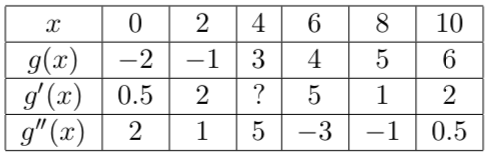
\includegraphics[scale=0.4]{Figures/tableg}
        \end{center}
Let $j(x) = g(14-4x)$.
\begin{enumerate}[(a)]
\item Use the values from the table to find a formula for $L(x)$, the linear approximation to $j(x)$ at $x = 2$.
\vspace{0.2in}
\item Find an approximate value for $j(2.25)$ using your formula for $L(x)$.
\vspace{0.2in}
\item Is your approximation in part (b) an overestimate or an underestimate? Circle your answer and give a justification of your answer.

\centering Overestimate \hspace{7mm} Underestimate \hspace{7mm} Not enough information 
\vspace{0.2in}
\end{enumerate}
\begin{solution}
  See \href{https://dhsp.math.lsa.umich.edu/exams/115exam2/f17/s1.pdf}{https://dhsp.math.lsa.umich.edu/exams/115exam2/f17/s1.pdf}
\end{solution}
\question (Winter 2018 Exam 2) %problem 9
Below is the graph of $h'(x)$.
\begin{center}
  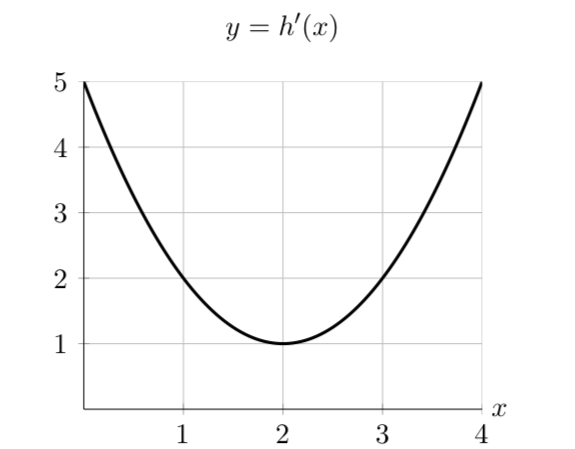
\includegraphics[scale=0.4]{Figures/Exam2W2018Problem9}
\end{center}
\begin{enumerate}[(a)]
\item Find a formula for the tangent line approximation $L(x)$ to the function $h(x)$ near $x = 2$ if the point $(2,-3)$ lies on the graph of $y = h(x)$. Your answer should not include the letter $h$.
\vspace{0.2in}
\item Use the tangent line approximation to $h(x)$ near $x = 2$ to approximate the value of $h(1.6)$.
\vspace{0.2in}
\item Is your approximation in part (b) an overestimate, an underestimate or is there not enough information to determine that?
\end{enumerate}
\begin{solution}
  See \href{https://dhsp.math.lsa.umich.edu/exams/115exam2/w18/s9.pdf}{https://dhsp.math.lsa.umich.edu/exams/115exam2/w18/s9.pdf}
\end{solution}
\end{questions}
\end{document}
%%% Local Variables:
%%% mode: latex
%%% TeX-master: t
%%% End:
